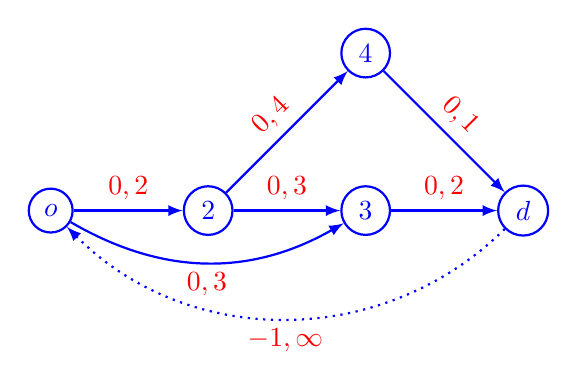
\begin{tikzpicture}[blue,thick,scale=2]
  \node[draw, circle] (V1) at (0, 0) {$o$};
  \node[draw, circle] (V2) at (1, 0) {$2$};
  \node[draw, circle] (V3) at (2, 0) {$3$};
  \node[draw, circle] (V4) at (2, 1) {$4$};
  \node[draw, circle] (V5) at (3, 0) {$d$};
  
  \draw[-latex] (V1) -- (V2) node[midway,above,red] {$0, 2$};
  \draw[-latex] (V2) -- (V3) node[midway,above,red] {$0, 3$};
  \draw[-latex] (V3) -- (V5) node[midway,above,red] {$0, 2$};
  \draw[-latex] (V2) -- (V4) node[midway,above,sloped,red] {$0, 4$};
  \draw[-latex] (V1) to[bend right] node[midway,below,red] {$0, 3$} (V3) ;
  \draw[-latex] (V4) -- (V5) node[midway,above,sloped,red] {$0, 1$};
  
  \draw[-latex,dotted] (V5) to[bend left=45, -|] node[midway, below, red] {$-1,\infty$} (V1) ;
\end{tikzpicture}

